\documentclass[a4paper,10pt]{article}
\usepackage{graphicx}
\usepackage[english]{babel}
\usepackage[latin1]{inputenc}
\usepackage[top=2.54cm,bottom=2.54cm, left=2.54cm, right=2.54cm]{geometry}


\begin{document}

\begin{titlepage}
\vspace*{-2cm}
%\centerline{\makebox[\textwidth]{\includegraphics[width=\paperwidth]{cover_page_header.png}}}
\vspace{2cm}
\center{\textbf{\Large{AERO40005 Laboratory Technique to Obtain Measurements for Strain, Stress and Hardness }}}
\center{\large{Ruairidh Scott-Brown}}
\center{\large{01734080}}
\vspace{2cm}          
\vspace{2cm}   

\vspace{7cm}

%\centerline{\makebox[\textwidth]{\includegraphics[width=\paperwidth]{cover_page_footer.png}}}
\end{titlepage}  

\newpage
\newpage
\addcontentsline{toc}{section}{List of Figures}
\listoffigures\newpage



\newpage
\section{Introduction}
%Introduction presents the significance of the experiment and explains the aims and objectives.
The mechanical response of a material under deformation can be quantified from the change in length under pressure. The degree to which the material reacts can be an indicator of the materials properties. The aim of the experiment was to use a variety of basic techniques to investigate the properties of six different materials. Copper, aluminium and brass specimens were loaded progressively under uniaxial tension, with a strain gauge attached, to evaluate their respective youngs modulus's. Specimens of aluminium, plastic and composite where stressed until failure to demonstrate the elastic and inelastic phases with the aluminium also being subject to indentation to measure the hardness and compare the results with the Tabor prediction.

\section{Theory and Background}
%In this section, you explain the scientific background of the experiment. Please cite the relevant references when you present theories, equations, etc. For further details about correct format of equations and symbols, see IC Aero Report Style Guide.
\subsection{Stress and Strain}
Stress is the ratio of force to cross sectional area of a plane cutting through a material. When acting in a uniaxial direction perpendicular to the cross sectional area, the stress acting on a material can be tensile (pull) where the material will lengthen in the same direction or compressive (push) where the material will shorten in the same direction. If the area of the material is only considered before deformation the stress is defined as the normal force per unit initial area.

\begin{equation}
 \label{Nominal Stress}
 \sigma_n = \frac{F_n}{A_0}
\end{equation}

Tension can can also act in parallel to the cross sectional area, defined as shear stress, causing the two sides of the material plane to slide over each other. 

\begin{equation}
 \label{Shear Stress}
 \tau = \frac{F}{A_0}
\end{equation}

Under stress a material can change shape and when the change in shape is considered in one direction on a plane it can be measured as the change in length. The ratio of change in length over the initial length is defined as strain. Again if the stress causing the strain is nominal stress the strain is also considered as the nominal strain.

\begin{equation}
 \label{Nominal Strain}
 \epsilon_n = \frac{\delta L}{L_0}
\end{equation}

However, when a material is acted upon by a shear stress the change in angle is considered over the change in length and the strain is measured as the difference between the initial angle minus angle separating the $x$ and $y$ axis.

\begin{equation}
 \label{Shear Strain}
 \gamma = \theta - \theta_0
\end{equation}

% This part goes in preamble
\newcommand{\dummyfig}[1]{
  \centering
  \fbox{
    \begin{minipage}[c][0.1\textheight][c]{0.7\textwidth}
      \centering{#1}
    \end{minipage}
  }
}

%% This part makes a figure
\begin{figure*}[h]
  \dummyfig{Dummy Figure Label} 
  \caption{Dummy figure caption}
  \label{fig:dummy}
\end{figure*}

The material cross sectional area will normally change when acted on by strain therefore with greater and greater strain the calculation for nominal stress becomes less accurate. However we can account for this with true stress which takes into account the varying cross sectional area.
 
\begin{equation}
 \label{True Stress}
 \sigma_t =\sigma_n(1 + \epsilon_n) 
\end{equation}

The same can be said for strain as the initial length will vary with as the addition of further strain therefore to compensate for the varying length true strain is measured.

\begin{equation}
 \label{True Strain}
 \epsilon_t = \ln{\frac{L}{L_0}}
\end{equation}

The relationship between stress and strain is unique to each material but follow some simple trends which can be used identify the material properties.

%% This part makes a figure
\begin{figure}[h]
  \dummyfig{Dummy Figure Label 1} 
  \caption{Dummy figure caption}
  \label{fig:dummy 1}
\end{figure}

At the first stage, strain increase linearly with stress where the constant of stress over strain is known as the modulus of elasticity (youngs modulus). Where the youngs modulus is a measure of a materials resistance to elastic strain. Stiff materials will have a high youngs modulus as it take a lot of stress to deform the them whereas flexible materials will have a low youngs modulus. This period of deformation is known as the elastic region as the material will return to the same state after the stress is removed.

\begin{equation}
 \label{Youngs Modulus}
 E = \frac{\sigma}{\epsilon}
\end{equation}

In the second stage, material will then enter the plastic stage where stress and strain no longer vary linearly. This results in permanent deformation of the material as when the stress is removed the material will no longer change back into its initial state. Note that when the material deforms back it will follows the gradient equal to the youngs modulus (the linear relationship between stress and strain is maintained. The transition between the elastic and plastic state is not sudden but the point at which marks the change is the yield point as its calculated as the stress (proof stress) which causes a permanent strain of 0.2\%. \par

The third stage is known as necking and comes after the ultimate tensile strength which indicates the largest stress that the material can take. Within this region the cross sectional area becomes significantly smaller (reducing the nominal stress but not the true stress) until the fracture point where the material splits in two.\newline

\begin{figure}[h]
  \dummyfig{Dummy Figure Label 1} 
  \caption{Dummy figure caption}
  \label{fig:dummy 1}
\end{figure}

\subsection{Hardness}
Hardness is the property of a material which describes its resistance to penetration. It's calculated as the ratio of indentation force over area where the area is considered to be the contact between the indenter and material projected on the plane perpendicular to the force. The indenter produces a small hemisphere region of compressive hydrostatic stress (same stress acts on all planes) which is proportional to the hardness of the material.

\begin{equation}
 \label{Hardness and Hydrostatic stress}
 H = \frac{F}{A} \approx \sigma_h
\end{equation}

Outside of this region the material undergoes plastic deformation where the yield point is reached but not under hydrostatic stress. As this suggest, the hardness of a material is related more towards the yield stress and plastic region of the stress strain relationship. Where a third of the hardness is evaluated as the stress associated with a 9\% of the total strain. 

\subsection{Strain Gauge}
%% This part makes a figure
\begin{figure}[h]
  \dummyfig{Dummy Figure Label 1} 
  \caption{Dummy figure caption}
  \label{fig:dummy 1}
\end{figure}

One of the pieces of equipment used to calculate the strain is a strain gauge. It works off the principle that the resistance of a conductive material (element) changes with strain. As a result, if a section of element is placed on the surface of a material the change in length of the material and element would be proportional (constant of proportionality is the gauge factor which is a material and geometry property $S$)  and therefore the change in resistance of the element can used to measure the strain applied to the material. 

\begin{equation}
 \label{Strain Gauge}
 \epsilon = \frac{\delta R/ R_o}{S}
\end{equation}

The circuit used to apply the strain gauge is known as a wheatstone bridge. It is used as the voltage across the circuit can take account for the change in resistance of the strain gauge but also cancels out resistance change due temperature change. To complete the circuit the has to go through an amplifier which increases the voltage by a constant factor know as the gain as the $V_out$ is normally in the region of milli volts.

\begin{equation}
 \label{Strain Gauge}
 \epsilon = \frac{4 \cdot V_out}{V_in \cdot S \cdot Gain}
\end{equation}










\section{Methodology}
\subsection{Strain Measurement with Strain Gauge}

%% This part makes a figure
\begin{figure}[h]
  \dummyfig{Dummy Figure Label 1} 
  \caption{Dummy figure caption}
  \label{fig:dummy 1}
\end{figure}
%% This part makes a figure
\begin{figure}[h]
  \dummyfig{Dummy Figure Label 1} 
  \caption{Dummy figure caption}
  \label{fig:dummy 1}
\end{figure}

Each sample had a strain gauge attached to the gauge portion of the dogbone in the axial direction and was placed in a hand operated tensile machine. The strain gauge was connected to a wheatstone bridge circuit where the $V_out$ was passed through a amplifier before being measured by a voltmeter.\newline

Experimental  Measurements
\begin{itemize}
\item[$\textendash$] dogbone diameter
\item[$\textendash$] gain of amplifier
\item[$\textendash$] gauge factor of strain gauge
\item[$\textendash$] $V_out$ at each load state.
\end{itemize}
Experiment Procedure
\begin{itemize}
\item[$\textendash$] Each specimen was loaded into the tensile machine with care taken not to induce any load.
\item[$\textendash$] The strain gauge was then connected to the wheatstone bridge circuit
\item[$\textendash$] The variable resistance of the wheatstone bridge was altered to produce and $V_out$ of zero with no load applied
\item[$\textendash$] A load increase of 0.5kN was applied via the tensile machine and the resulting change in voltage was noted.
\item[$\textendash$] Once the load reached 3.5kN the specimen was steadily unloaded.
\item[$\textendash$] This process was repeated for each specimen.
\end{itemize}

\subsection{Stress Till Failure}

%% This part makes a figure
\begin{figure}[h]
  \dummyfig{Dummy Figure Label 1} 
  \caption{Dummy figure caption}
  \label{fig:dummy 1}
\end{figure}
%% This part makes a figure
\begin{figure}[h]
  \dummyfig{Dummy Figure Label 1} 
  \caption{Dummy figure caption}
  \label{fig:dummy 1}
\end{figure}

The dogbone sample was mounted within a hand  operated tensometer which consisted of a resistive load cell which recorded the force applied to the sample and a mechanical extensometer which recorded the displacement of the tensile machines cross heads.

Experimental  Measurements
\begin{itemize}
\item[$\textendash$] cross sectional area of dogbone
\item[$\textendash$] initial length of gauge portion
\item[$\textendash$] stretch of specimen
\item[$\textendash$] force applied to  specimen
\end{itemize}
Experimental  Procedure
\begin{itemize}
\item[$\textendash$] The specimen was loaded into the tensile machine with care not to induce load.
\item[$\textendash$] Progressive load was applied slowly to the specimen until failure.
\item[$\textendash$] This process was repeated for each specimen. 
\end{itemize}

\subsection{Hardness}
%% This part makes a figure
\begin{figure}[h]
  \dummyfig{Dummy Figure Label 1} 
  \caption{Dummy figure caption}
  \label{fig:dummy 1}
\end{figure}
%% This part makes a figure
\begin{figure}[h]
  \dummyfig{Dummy Figure Label 1} 
  \caption{Dummy figure caption}
  \label{fig:dummy 1}
\end{figure}



\section{Results and Discussions}
%Results and discussions is the main part of the report in which key findings are presented in graphs and tables and discussed. It is very important to refer to all figures and tables in the text. A number of graphs and tables without relevant individual explanation cannot be considered as an acceptable results section. You should quantitatively analyse errors and uncertainties in this section.
\subsection{Strain Measurement and Strain Gauge}
\subsubsection{Graphs}
%Graphs should be clear and readable with a caption and figure number below. For further details about graphs, see IC Aero Report Style Guide.

The raw results from the experiment as seen in figure[\ref{Fig1}], show the three specimens of aluminium, copper and brass under loading and unloading stress. The rate of change of force with respect to amplified voltage for loading can be seen to be constant. This shows that the material undergoes only elastic deformation as the loading phase shows no sign of reaching a yield point and the unloading phase reaches close to the initial voltage (i.e. describes a scenario with no plastic/permanent deformation). 
\begin{figure}[htb]
\centering
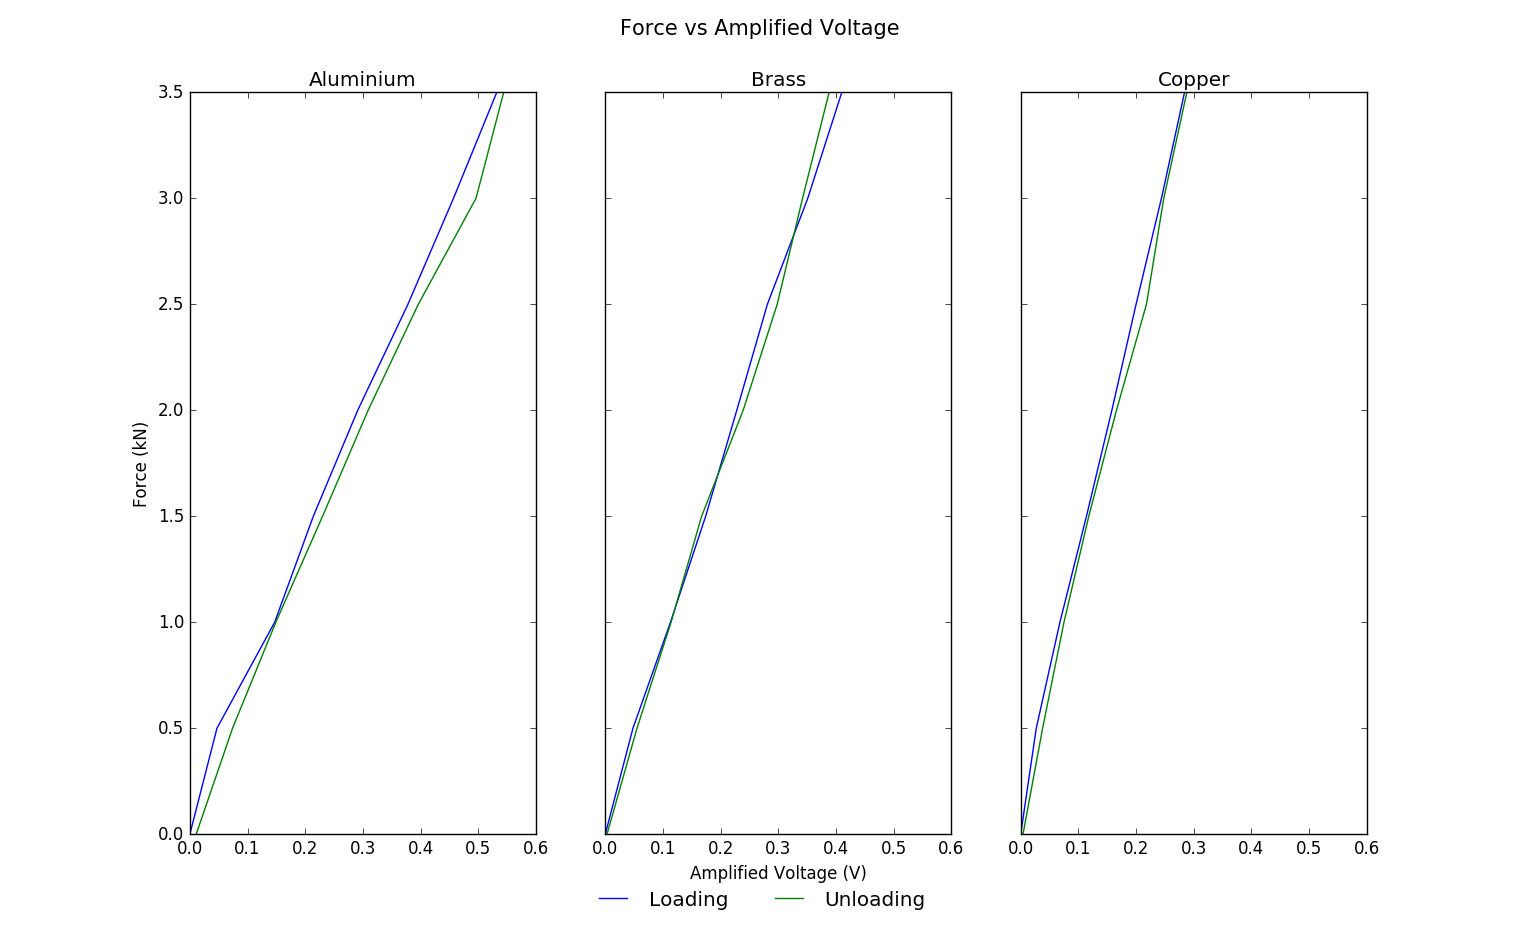
\includegraphics[width=\textwidth]{figure_3.png}
\caption{Force applied via the tensile meter (kN) vs. the amplified voltage from the wheatstone bridge (V).}
\label{Fig1}
\end{figure}

The nominal strain can be calculated from equation[\ref{Nominal Strain}] and related to the nominal stress calculated equation[\ref{Nominal Stress}] as shown in figure[\ref{Fig2}] 

\begin{figure}[htb]
\centering
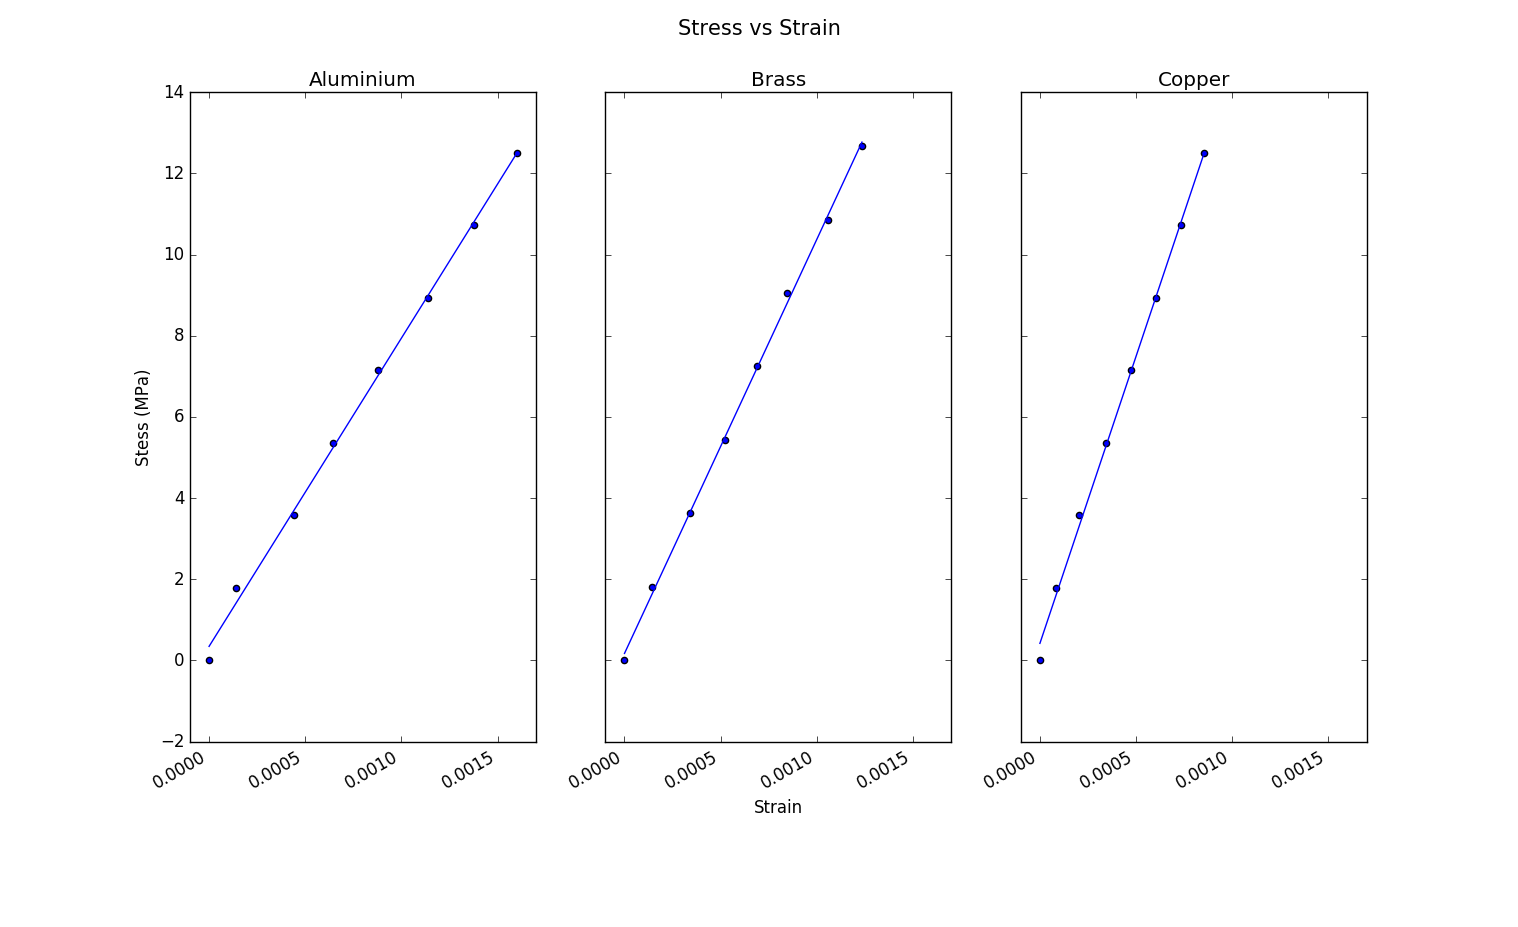
\includegraphics[width=\textwidth]{figure_4.png}
\caption{Nominal stress (MPa) vs.  nominal strain acting on each specimen with a line of best fit plotted to estimate the youngs modulus ($Nm^{-2}$). Note: the errors have been neglected due to scale but are present in figure[\ref{Fig4}] and figure[\ref{Fig5}].}
\label{Fig2}
\end{figure}

Figure[\ref{Fig2}] further supports the idea that the samples are elastically deformed as the relationship between stress and strain is linear. This allows the results to be evaluated through the use of equation[\ref{Youngs Modulus}] i.e. Hooke law to identify the youngs modulus and to therefore describe the degree of stiffness of each material. The difference between the loading and unloading phases can clearly be seen in figure[\ref{Fig2}] and can't be accounted for in the errors from figure[\ref{Fig5}] or figure[\ref{Fig6}]. The unloading phase youngs modulus is less than the loading phases modulus for aluminium and copper however the youngs modulus for the unloading phase for brass was higher than the loading phase thus proving that there isn't a systematic uncertainty in the experiment solely responsible for error. Human error in reading the analogue force meter could have come into account which would vary the reliability of the force measurements. 
\subsubsection{Tables}
%Tables should be accompanied by a caption and table number above. For further details about tables and tabulation of data, see IC Aero Report Style Guide.
\begin{figure}[!]
\centering
\caption{Raw results from the tensile meter and strain gauge}
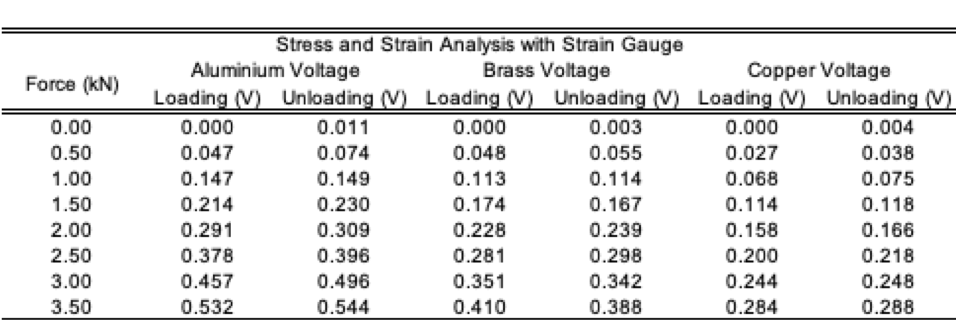
\includegraphics[width=\textwidth]{Picture_raw_strain_gauge.png}
\label{Fig3}
\end{figure}

\begin{figure}[!]
\centering
\caption{Processed data from the tensile meter to calculate stress}
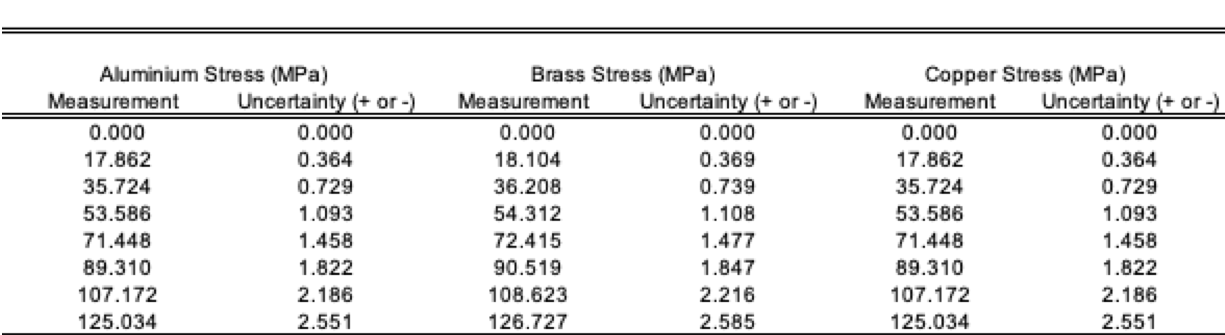
\includegraphics[width=\textwidth]{processed_strain_gauge.png}
\label{Fig4}
\end{figure}

\begin{figure}[!]
\centering
\caption{Processed data from the voltmeter to calculate the strain during the loading phase}
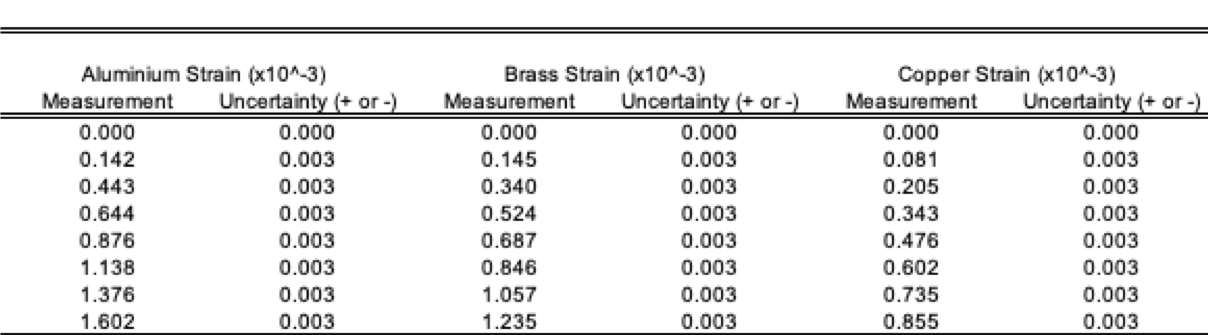
\includegraphics[width=\textwidth]{processed_stress_gauge.png}
\label{Fig5}
\end{figure}

\begin{figure}[!]
\centering
\caption{youngs modulus's for the loading and unloading phase}
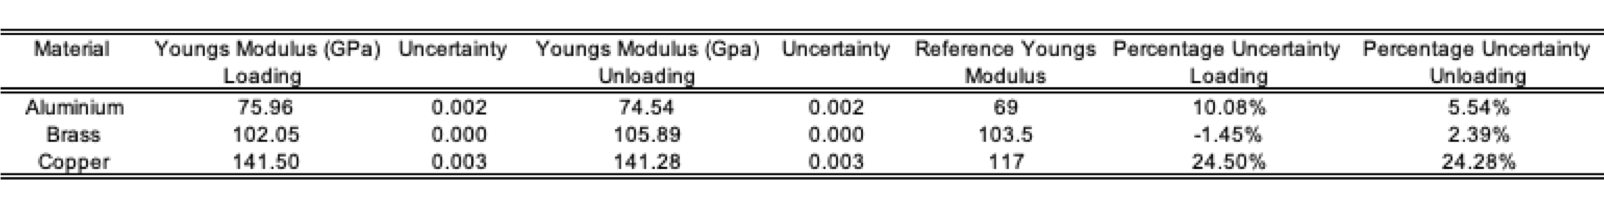
\includegraphics[width=\textwidth]{final_result.png}
\label{Fig6}
\end{figure}

The experimental results from figure[\ref{Fig6}] can be compared with the reference values of the materials [ ]. When it comes to aluminium and copper the the experimental results were greater than expected. However, the brass results varied as the loading phase produced a lower youngs modulus but the unloading produced a higher youngs modulus. In fact, the average between the loading and unloading youngs modulus values for brass equals 103.97 MPa which has a percentage error of 0.4\% with respect to the reference value 103.5 MPa. \newpage

%\subsubsection{Equations}
%Equations should be centered and numbered in the right end of the line. For further details about equations, symbols and units, see IC Aero Report Style Guide.
%\begin{equation}
 %\delta=\frac{FL}{AE}
 %\end{equation}

\subsection{Failure Under Tension}
\subsubsection{Graphs}

\begin{figure}[htb]
\centering
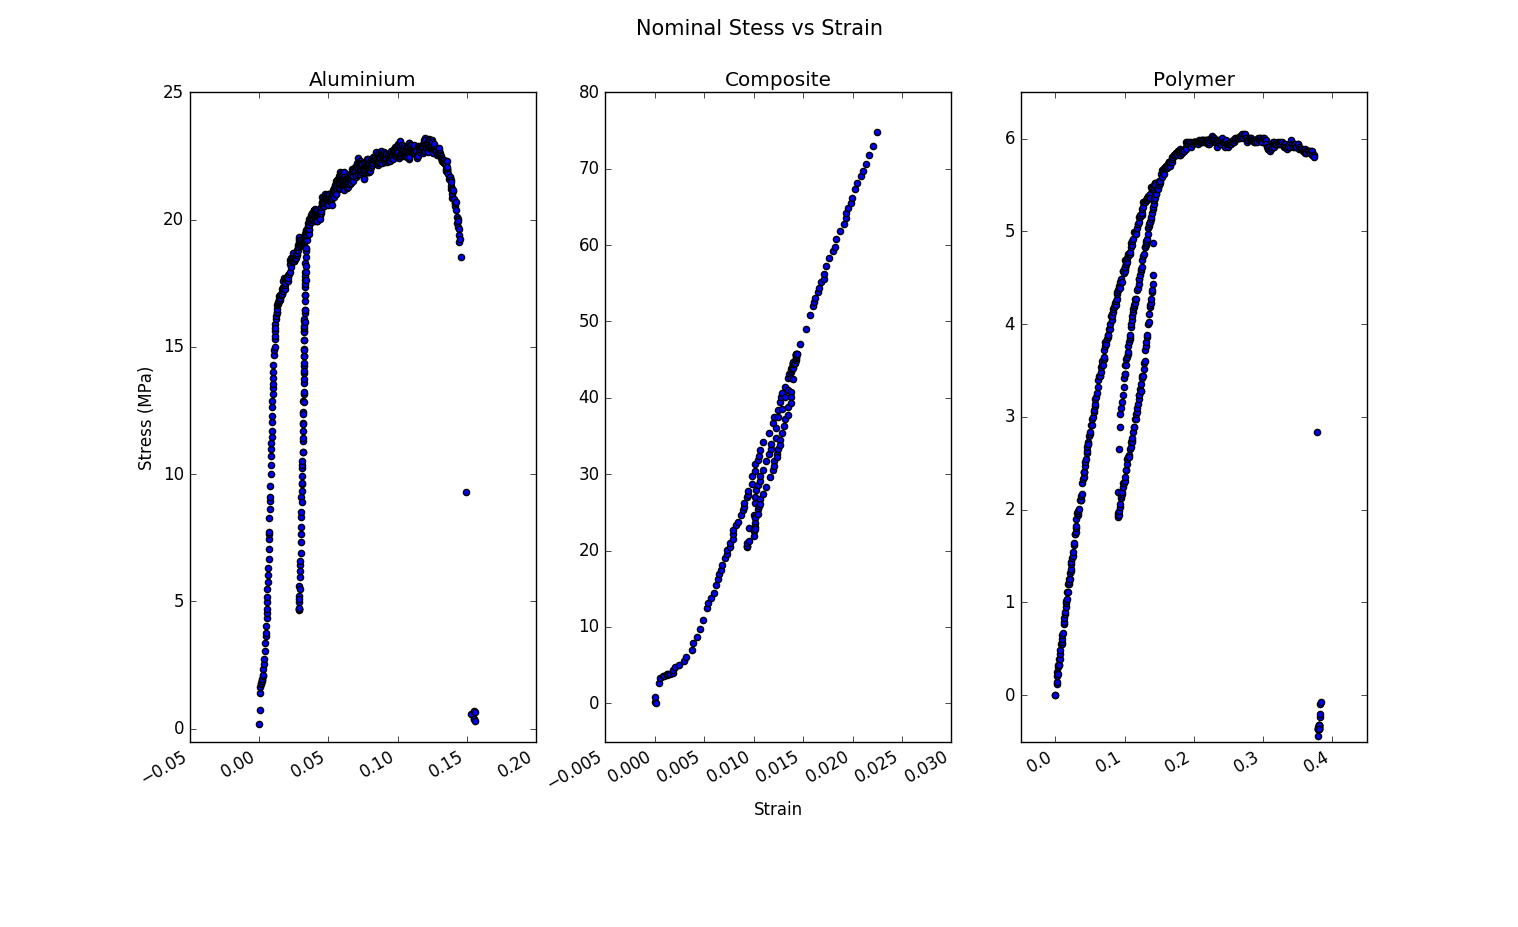
\includegraphics[width=\textwidth]{figure_1.png}
\caption{Nominal stress (MPa) vs. nominal strain on each sample (aluminium, composite, polymer) with an unloading phase}
\label{Fig7}
\end{figure}
 
 Within figure[\ref{Fig7}] the composite doesn't seem to have undergone plastic deformation due to the relationship between stress and strain remaining linear up to the fracture point. This describes the composite as brittle as it wont bend under high stress only break or fracture.This is further supported as the fracture point of the composite is relatively high compared to the aluminium and polymer. The aluminium sample has a clear\par
 When the composite and polymer samples go under unloading and reloading the relationship between stress and strain doesn't remain linear and don't match the elastic phase of the respective materials. Whereas, the aluminium handles the unloading and reloading phases as expected with the relationship between stress and strain matching the youngs modulus.\\[8pt]

\begin{figure}[!]
\centering
\includegraphics[width=0.7\textwidth]{figure_2_pol.png}
\caption{True stress vs. true strain against nominal stress vs. nominal strain of the polymer specimen with a line of best fit that estimates the youngs modulus.}
\label{Fig8}
\end{figure}

Within figures[\ref{Fig8}][\ref{Fig9}][\ref{Fig10}] the true stress data points are higher during the plastic deformation stage of each material. This is expected as the nominal stress doesn't take into account the change in area with increased strain. If the material starts to undergo stress it tends to lengthen in the direction of the stress and shorted in the perpendicular axis (the plane in which we calculate  the area) therefore if we keep the area constant (equation[\ref{Nominal Stress}]) then the resulting stress will seem to be smaller than if we take in consideration the area change (equation[\ref{True Stress}]).\\[8pt]
Both figures[\ref{Fig9}][\ref{Fig10}] have a curves at the start of their stress strain relationships whereby strain is recorded with very little stress. This is caused by slack between the tensile meter grips and the dogbone samples and has been accounted for in the calculations for the youngs modulus.
\begin{figure}[!]
\centering
\includegraphics[width=0.7\textwidth]{figure_2_al.png}
\caption{True stress vs. true strain against nominal stress vs. nominal strain of the aluminium specimen with a line of best fit that estimates the youngs modulus and estimation for the hardness using Tabor prediction. (Toughness from true stress strain curve = 705 MPa and from the nominal stress strain curve = 650 MPa)}
\label{Fig9}
\end{figure}

\begin{figure}[!]
\centering
\includegraphics[width=0.7\textwidth]{figure_2_comp.png}
\caption{True stress vs. true strain against nominal stress vs. nominal strain of the composite specimen with a line of best fit that estimates the youngs modulus.}
\label{Fig10}
\end{figure}

\subsubsection{Tables}

\begin{figure}[!]
\centering
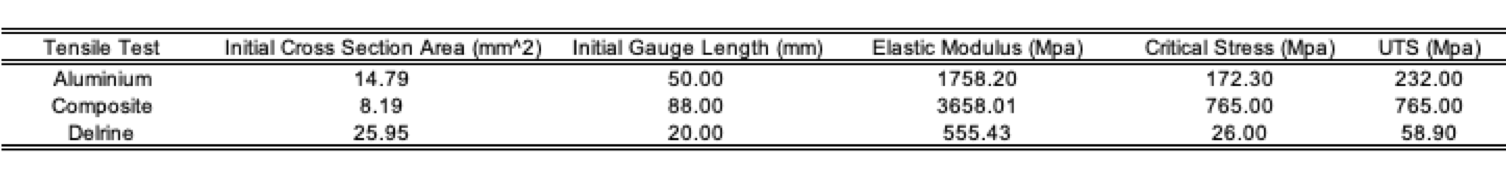
\includegraphics[width = \textwidth]{harndess_1.png}
\caption{Dimensions of dogbone specimen as well as calculated material properties from the graph. Ultimate Tensile Strength (UTS}
\label{Fig10}
\end{figure}
\begin{figure}[!]
\centering
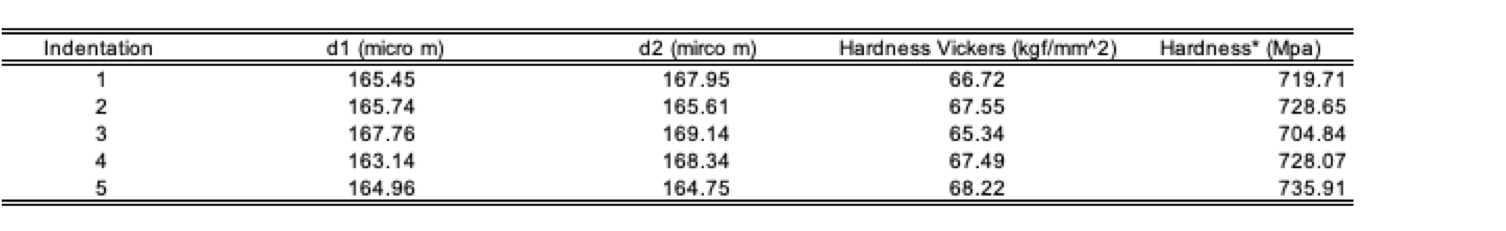
\includegraphics[width = \textwidth]{hardness_2.png}
\caption{Raw and processed results from the hardness testing. d1 and d2 represent the diagonal distance across the indentation diamond from the vickers indenter.}
\label{Fig10}
\end{figure}
\begin{figure}[!]
\centering
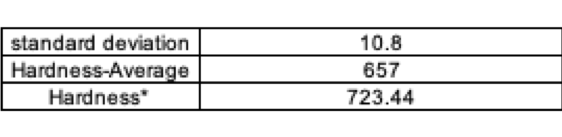
\includegraphics[width = 0.5\textwidth]{hardness_3.png}
\caption{Hardness values in MPa
The value calculated from the hardness experiment doesn't match the results from the Tabor prediction in figure[\ref{Fig9}]}
\label{Hard}
\end{figure}




\newpage
\newpage
\section{Conclusions}
%Here, you draw conclusions based on the presented results. In conclusions, you should discuss the success of the experiment and address aims and objectives of the experiment
The youngs modulus's calculated from the strain gauge experiment figure[\ref{Fig6}] ranged in accuracy but the measurement for the brass sample was particularly accurate with a percentage error of 0.4\%. \par When it came to the hardness experiment the results from the tabor prediction (figure[\ref{Fig9}]) and indentations test (figure[\ref{Hard}]) didn't agree with the indentation test producing higher results than the tabor

\end{document}